\documentclass[a4paper,10pt]{article}
\usepackage[utf8]{inputenc}
\usepackage{amsmath}
\usepackage{graphicx}
\usepackage{epsfig}
\usepackage[english]{babel}
\usepackage{url}
\usepackage{epstopdf}
\usepackage{subfig}
\usepackage{graphicx}
\usepackage{enumerate}
\usepackage{appendix}
%\usepackage{anysize}
%\marginsize{1cm}{1cm}{1cm}{1cm}
\title{\textit{IEE3853} Detectores para Astronomía (I-2012)}
\author{\textbf{Tarea 04 – Diseño del sistema de detección para un Imager} \\Norman F. Sáez\\nfsaez@uc.cl}

\date{2012/07/07}

\begin{document}
%\input{portada}
\maketitle
\section*{Introducción}

El presente documento especifica sistema de detección para el telescopio ESO 1
metro, en donde el instrumento a utilizar es Imager.  Los requerimientos
especificados fueron los siguientes:

\begin{itemize}
\item Especificar el CCD científico a utilizar.

\item Predecir readout noise, dark current y readout time.

\item Estimar si el diseño óptico es adecuado o es preferible modificarlo, para
el detector seleccionado. En caso de modificación, especifique los
requerimientos para el nuevo diseño óptico.

\item Estimar los tiempos de exposición para diversos filtros considerando la
eficiencia cuántica del CCD seleccionado y la obtención de una SNR de al menos
10. Analice filtros del tipo SDSS4 (Sloan Digital Sky Survey) para su análisis.

\item Especificar los requerimientos de enfriamiento criogénico, en particular
temperatura de operación. Sugerir posibilidades de criogenia.
\end{itemize}

Las siguientes secciones muestran como se intenta satisfacer las necesidades que se especificaban en la tarea.


%PREGUNTA 1
\section{Especificar el CCD científico a utilizar}
Parámetros del sistema:
\begin{itemize}
\item Field of View del instrumento = $14 '$
\item Diámetro Plano Focal = $30.8 [mm]$
\item Escala en el plano focal = $\frac{FoV}{Diametro\ Plano\ Focal} = 0.4545 ['/mm]$
\item Field of View requerido: $5'$ en x
\item Field of View requerido: $5'$ en y
\item Dimensiones del detector: $\frac{5'}{0.4545['/mm]} = 11 [mm]$ en x
\item Dimensiones del detector: $\frac{5'}{0.4545['/mm]} = 11 [mm]$ en y
\end{itemize}
Entonces el detector debe tener un tamaño de $11x11[mm]$.  Tamaño imagen de la
PSF en el plano focal: $\frac{0.00833'}{0.4545 ['/mm]} = 0.01833[mm] = 18.33516
[\mu m]$, utilizando el dato de Optimal Sampling, podemos obtener cuanto tiene
que ser el tamaño del píxel: $\frac{18.33516}{3} = 6.111 [\mu m]$.

Con los datos obtenidos, se necesita como mínimo:
\begin{itemize}
\item CCD $11x11[mm]$ como tamaño máximo del CCD.
\item Tamaño mínimo de cada píxel $6.11 [\mu m]$.
\end{itemize}

Con estos datos no es posible tener un CCD desde la pagina del proveedor. Por
lo que se intentara buscar uno similar y ajustar algunos parámetros del
instrumento.
Los datos obtenidos para determinar que no existe un CCD que reúna las características adecuadas, se muestran en figura \ref{fig:p1} 
\begin{figure}[ht!]
  \centering
  \subfloat[Tabla de datos siguiendo especificaciones]{\label{fig:p1_a}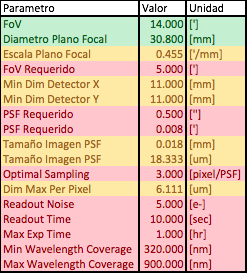
\includegraphics[width=0.5\textwidth]{img/img1}}
  ~ 
  \subfloat[Simbología]{\label{fig:p1_b}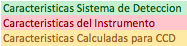
\includegraphics[width=0.3\textwidth]{img/simbologia}}
  ~ 
  \caption{Tabla de datos y simbología de acuerdo a las especificaciones}
  \label{fig:p1}
\end{figure}



%PREGUNTA 2
\section{Estimar si el diseño óptico es adecuado o es preferible
modificarlo,para el detector seleccionado. En caso de modificación, especifique
los requerimientos para el nuevo diseño óptico.} 

Dado que no existían CCD que se ajustara con las especificaciones, se plantea la
siguiente solución:
\begin{itemize}
\item Disminuir escala en el plano focal del instrumento
\end{itemize}

Para ello, se necesita:
\begin{itemize}
\item Disminuir el Field of View.
\end{itemize}
o bien:
\begin{itemize}
\item Aumentar el diámetro.
\end{itemize}

Luego, se seleccionaron cámaras que tuvieran el diámetro focal cercano a 30.8.
Las mejores cámaras escogidas fueron:
\begin{itemize}
\item CCD40-42,  Image Area: 27.64x27.64 $[mm]$ ( o 764.411904 $[mm^2]$)
\item CCD55-30,  Image Area: 25.92x27.94 $[mm]$ ( o 724.3344   $[mm^2]$)
\item CCD230-42, Image Area: 30.96x30.72 $[mm]$ ( o 951.0912   $[mm^2]$)
\end{itemize}
Se estudia la opción de elegir CCD40-42 debido Field of View cercano a 30.8.
Para utilizar se tiene que ajustar el Field of View de las especificaciones, de
tal manera que sea coherente con el tamaño máximo que pueden tener los píxeles.
Ver figura \ref{fig:ccd40p2} para revisar los datos obtenidos.
\begin{figure}[ht!]
  \centering
  \subfloat[CCD40-42 Tabla de datos ajustando especificaciones]{\label{fig:ccd40p2_a}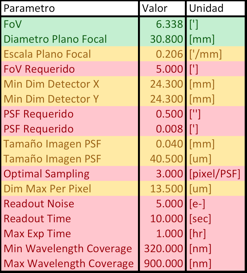
\includegraphics[width=0.5\textwidth]{img/ccd40-42}}
  ~ 
  \subfloat[Simbología]{\label{fig:ccd40p2_b}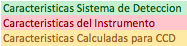
\includegraphics[width=0.3\textwidth]{img/simbologia}}
  ~ 
  \caption{CCD40-42}
  \label{fig:ccd40p2}
\end{figure}

Otra posibilidad es elegir CCD55-30. En este caso también es necesario
modificar el Field of View de acuerdo a las especificaciones del detector, al igual que en CCD40-42.  Ver
figura \ref{fig:ccd50p2}
\begin{figure}[ht!]
  \centering
  \subfloat[CCD55-30 Tabla de datos ajustando especificaciones]{\label{fig:ccd50p2_a}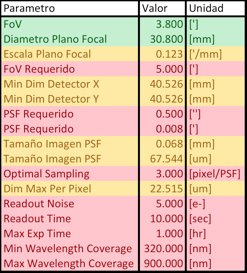
\includegraphics[width=0.5\textwidth]{img/ccd55-30}}
  ~ 
  \subfloat[Simbología]{\label{fig:ccd50p2_b}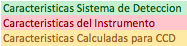
\includegraphics[width=0.3\textwidth]{img/simbologia}}
  ~ 
  \caption{CCD55-30}
  \label{fig:ccd50p2}
\end{figure}

La ultima opción a considerar es CCD230-42, debido a que su image view es
cercano a 30.8 y dentro de las CCD seleccionadas, es la que tiene mayor image
view. Se ajusta Field of View para que cumpla con las especificaciones de la
cámara y también el diámetro en el plano focal. De acuerdo a las
especificaciones de la cámara, se recalcula el Field of View para que cumpla
los valores tanto de tamaño de los píxeles así como el tamaño de la cámara, y
se aumenta en 0.2[mm] el diámetro en el plano focal para calzar las
especificaciones del detector.
Ver figura \ref{fig:ccd230p2}
\begin{figure}[ht!]
  \centering
  \subfloat[CCD230-42 Tabla de datos ajustando especificaciones]{\label{fig:ccd230p2_a}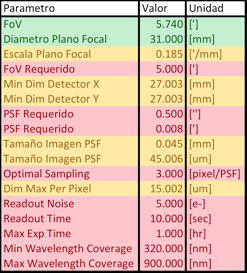
\includegraphics[width=0.5\textwidth]{img/ccd230-42}}
  ~ 
  \subfloat[Simbología]{\label{fig:ccd230p2_b}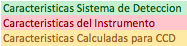
\includegraphics[width=0.3\textwidth]{img/simbologia}}
  ~ 
  \caption{CCD230-42}
  \label{fig:ccd230p2}
\end{figure}

Hasta el momento, se consideraran todos estos detectores como detectores
validos, ya que para todos ellos hay que hacer modificaciones al diseño
original. En las siguientes preguntas, se intentara decir por la mejor opción
cumpliendo las características ya requeridas.
%PREGUNTA 3
\section{Predecir readout noise, dark current y readout time}
Dada las características presentadas en la pregunta 2 y el datasheet de cada
detector, se revisa a continuación spectral range, readout noise, dark current y readout
frequency, para cada caso:
\subsection{Spectral Range}
\begin{figure}[ht!]
  \centering
  \subfloat[Spectral range para todas las cámaras propuestas]{\label{fig:spectral}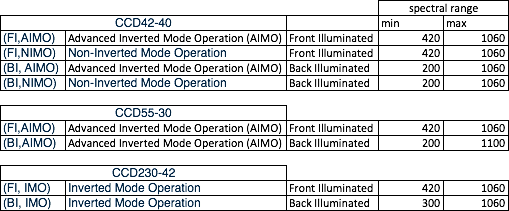
\includegraphics[width=0.8\textwidth]{img/spectral_range}}
  ~ 
  \caption{Spectral Range en $[nm]$}
  \label{fig:p3_b}
\end{figure}
Dada los requerimientos, solamente es posible utilizar detectores del tipo Back Illuminated.
\newpage
\subsection{Readout Frequency}
Podemos estimar readout frequency de la siguiente manera:
\begin{description}
\item [pixels]: Número de píxeles total de la cámara
\item [tiempo]: Máximo tiempo de lectura requerido
\item [amplificadores]: Número de amplificadores de salida
\end{description}

Dado los parámetros anteriores el readout frequency se puede calcular: 
\begin{align*}
readout\ frequency &= \frac{pixels}{tiempo*amplificadores}\\
\end{align*}
Se puede ver figura \ref{fig:p3} para  cada una de las cámaras
\begin{figure}[ht!]
  \centering
  \subfloat[CCD40-42]{\label{fig:ccd40p3}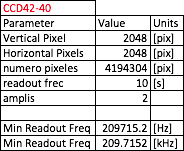
\includegraphics[width=0.3\textwidth]{img/ccd40-42p3}}
  ~ 
  \subfloat[CCD55-30]{\label{fig:ccd50p3}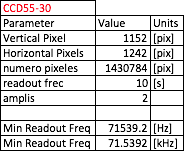
\includegraphics[width=0.3\textwidth]{img/ccd55-30p3}}
  ~ 
  \subfloat[CCD230-42]{\label{fig:ccd230p3}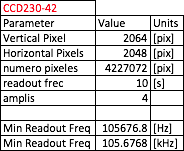
\includegraphics[width=0.3\textwidth]{img/ccd230-42p3}}
  ~ 
  \caption{Readout Frequency para cada cámara}
  \label{fig:p3}
\end{figure}

\subsection{Readout Noise}
\begin{figure}[ht!]
  \centering
  \subfloat[Readout Noise para todas las cámaras propuestas]{\label{fig:readout}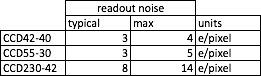
\includegraphics[width=0.4\textwidth]{img/readoutnoise}}
  ~ 
  \caption{Readout Noise}
  \label{fig:p3_a}
\end{figure}

Dada los requerimientos y en base a figura \ref{fig:p3_a}  no es posible
utilizar CCD230-42, debido a que supera el readout noise requerido. Por lo
tanto se descarta. 

\subsection{Dark Current}
Dark current para todas las cámaras propuestas se puede revisar en \ref{fig:p3_c}
\begin{figure}[ht!]
  \centering
  \subfloat[Dark Current para todas las cámaras propuestas]{\label{fig:darkcurrent}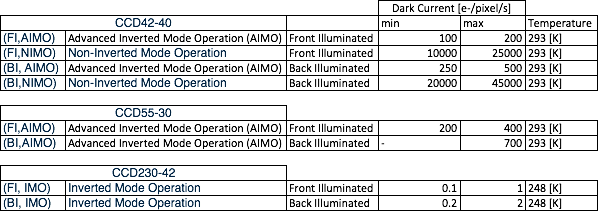
\includegraphics[width=0.8\textwidth]{img/darkcurrent}}
  ~ 
  \caption{Dark Current}
  \label{fig:p3_c}
\end{figure}

Cabe señalar que no es posible hacer una comparativa con todos los modelos,
debido a que cada una de las cámaras cambia dark current dependiendo de la
temperatura.

Debido a los datos anteriores, se descarta CCD40-42, debido a su alto readout
noise. Además, y debido a las características del tamaño del píxel requerido y
a las modificaciones en el Field of View, se descarta la utilización de
CCD55-30. La mejor opción es CCD40-42. El Field of View es el mayor de todos y
además Image Area es mayor a CCD55-30, su mas cercano rival. A favor de
CCD40-42 es el tamaño del píxel comparando con CCD55-30. (CCD55-30 tenia un
píxel de tamaño $\pm 22 [\mu m]$ comparado con el tamaño del píxel de CCD40-42
que es de $\pm 15 [\mu m]$ .
%PREGUNTA 4
\section{Estimar los tiempos de exposición para diversos filtros considerando la
eficiencia cuántica del CCD seleccionado y la obtención de una SNR de al menos
10. Analice filtros del tipo SDSS4 (Sloan Digital Sky Survey) para su análisis.}
Para poder analizar esta pregunta es necesario tener en consideración la figura \ref{fig:p4}

%\begin{figure}[ht!]
%  \centering
%  \subfloat[QE v/s Wavelength]{\label{fig:p4_a}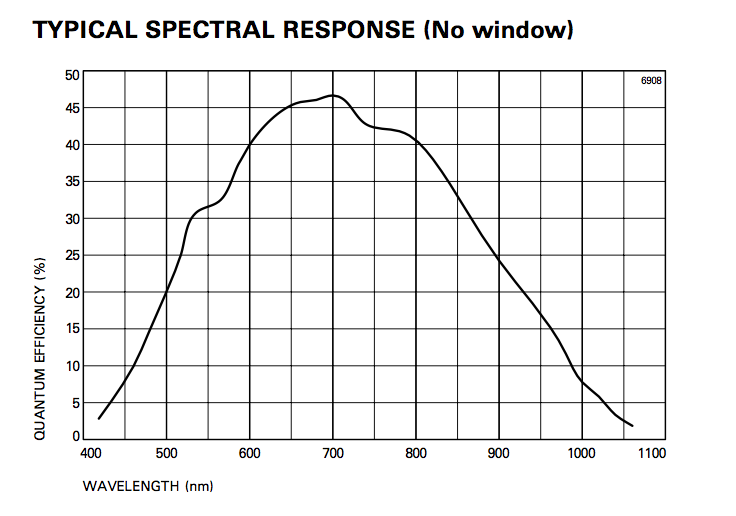
\includegraphics[width=0.8\textwidth]{img/img6}}
%  ~ 
%  \caption{Quantum Efficiency (\%) v/s Wavelength ($[nm]$)}
%  \label{fig:p4}
%\end{figure}

%PREGUNTA 5
\section{Especificar los requerimientos de enfriamiento criogénico, en particular
temperatura de operación. Sugerir posibilidades de criogenia.}


\end{document}

